\pdfbookmark[1]{Results}{results}
\chapter{Results. data treatment and discussion}


\section{Resonators}
First we make an overview of our resonator frequencies:
\begin{figure}
    \centering
    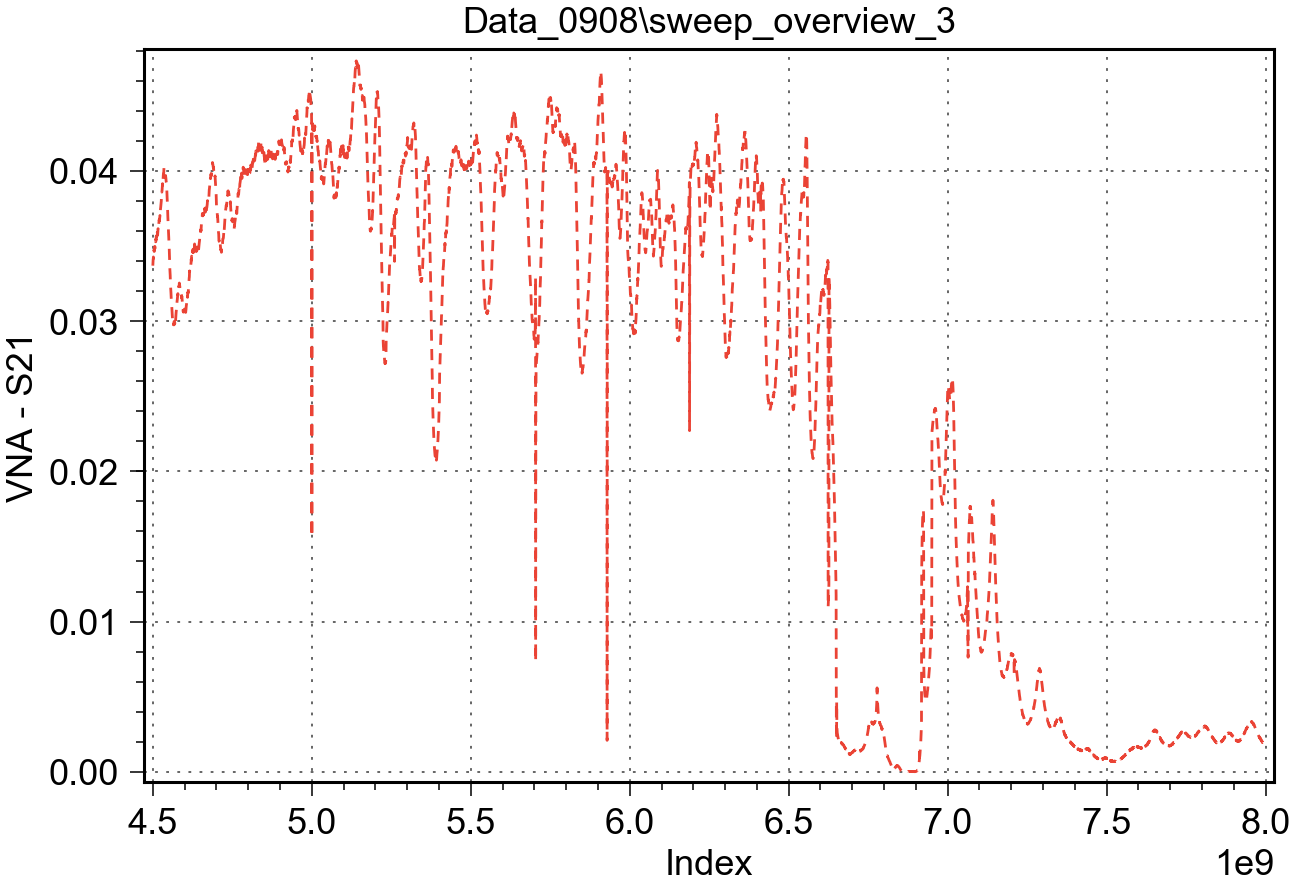
\includegraphics[width = 13cm]{Images/sweep_overview_3.png}
    \caption{This is a classical sweet overview of a resonator chip. At around 7 GHz, you see the frequency of the TWPA amplifyer}
    \label{fig:sweep_overview}
\end{figure}
We can then zoom in on each peak, and make a powerscan. notice that at aroun 7 GHz, we can see the TWPA amplifeyer frequency. 
\subsection{The fitting of the resonator peak}
We fit the resonator peak to a lorentzian. The width is given by: 
\begin{equation}
    w \propto \frac{w}{Q_t}
\end{equation}
Check the equations and cite the right papers. 
where the Qt is the total quality factor of our system. 

The maximum height depend on the capacitance (determines how big a fraction of photons is comming into our resonator) but it is also determined by how many of our electrons is Qe electrons meaning they go back into ours system: 
\begin{equation}
    I_{max} \propto \frac{Q_e}{Q_e + Q_i}
\end{equation}